\documentclass{article}

\usepackage{graphicx}
\usepackage{cleveref}
\usepackage{natbib}

% macros (move to its own file when we have a macro).

\begin{document}

\title{POPLMark goes Concurrent!\\Challenge problems for process calculi and behavioural types}

\maketitle

\begin{abstract}
  The publication of POPLMark spearheaded the era of publishing formal
  proofs alongside with new research. This fostered an era of
  high-quality and high-assurance proofs at top venues for programming
  language research. This paper simultaneously acknowledges the impact
  of the original POPLMark challenge, and proposes a new benchmark
  intended to stimulate the research and dissemination of techniques
  that address the particular challenges of process calculi and
  behavioural type systems. In this work we propose three challenge
  problems concerning to process calculi and name passing, linearity
  in behavioural type systems, and coinductive reasoning for process
  algebras.
\end{abstract}

\section{Introduction}

In recent years, at programming language venues there is the growing
expectation that the theoretical results of a paper are formalised in
a proof assistant. % rephrase
For this purpose, and to get the community on track the
POPLMark~\cite{Pierce:2005} challenge was proposed. Since then the
number of formal proofs accompanying papers has grown (add some POPL
statistics here). However, formal proofs are not equally spread in any
field, and the key contribution of challenges like POPLMark is to help
develop the necessary momentum and culture to be able to formalise
results. It has been a long time since the original challenge, and
many changes have happened. Particularly, POPLMark and any challenge
cannot address every conceivable technique. Challenges have to be
simple so that the techniques are not shadowed by technical details
and also feasible to implement without heroic efforts. In that vein,
it is apparent that new challenges are needed, work like POPLMark
Reloaded~\cite{Pientka:2019} strives to extend the scope of the
original challenge to proofs using logical relations. This technique
is crucial to many current developments.

In this work, we address another expansion of scope for such
challenges, going from the $\lambda$-calculus to process calculi like
the $\pi$-calculus and session type systems (and other behavioural
type systems). These systems require particular insights to implement.
We have identified three key aspects. First, the idea of scope
extrusion in name passing calculi. This generalises the idea of
binders in ways that techniques that were adequate for
$\lambda$-calculus binders are not so for name passing systems.
Second, session types in particular, and behavioural types in general
often depend on linearity in their type systems. The formalisation of
linear type systems posses a challenge given that it is not uniformly
well supported among the many proof assistants. Finally, processes in
concurrent systems often contain infinite behaviour that is modelled
with coinduction. This technique is used to reason about
(bi)similarity between processes, the equivalence of their traces, or
subtyping between infinite trees of possible behaviours. This
challenge concentrates on those issues.

In this work we propose a challenge where each part independently
exercises one of the three areas, however it is often the case that a
problem requires more than one of these techniques simultaneously. In
this work, we explore them in isolation, in order to facilitate the
implementation of smaller solutions. Concretely, we do not address the
idea of how to combine these techniques, leaving the discussion of
that to the future when we have collected enough entries to these
problems.

We do not claim in this work that these problems have never been
approached and formalised before. In fact, the contrary is true. All
of these problems have been addressed in several forms. This motivates
this challenge to enable an easier comparison between solutions (since
they all implement the same challenge), and in a setting that is
simple enough to not be distracting, yet complex enough that we can
compare strengths and weaknesses of each.

The rest of this paper is structured in the following way:
\cref{sec:rationale} expands on the rationale for the selected
challenge problems. Then \cref{sec:problems} presents the problems. We
discuss the solutions in \cref{sec:solutions}, in particular
\cref{sec:tutorial} walks through a tutorial solution. And finally
\cref{sec:conclusion} presents some conclusions and it contains a call
to action to invite the submission of new solutions.

\section{Rationale for choosing the problems}\label{sec:rationale}

This section is not (at least initially) meant to be in the final
manuscript but it is to document some reasoning for choosing
appropriate problems. The idea is to explore three areas, scope
extrusion in name passing calculi, linearity requirements in
behavioural types, and finally coinductive reasoning, in trace
equivalence, (bi)similarity, or subtyping in the presence of
recursion.

The idea is to have three small problems in the aforementioned
subjects that are independent of each other and that are easy to
understand and to implement. This is important so we have more
entries. They have to be small so it is not a lot to read, and
independent so people may choose to implement only one of them, or
work on them in any order.

Finally, it is important to mention in the rationale for problems that
the key aspects are:
\begin{itemize}
\item Scope extrusion
\item Linearity
\item Coinduction
\end{itemize}

But the exact presentation of the concrete problems should be somewhat
flexible. In the sense that the use of certain techniques or tools may
require changing the presentation of the system to fit the technique.
These changes should be allowed, and even encouraged, but the result
should be ``obviously'' the same system and there should be a
rationale for the changes in presentation. That way we could not only
see valid techniques but also what presentation of the rules to use
and the rationale to chose a particular approach.

\section{The challenge problems} \label{sec:problems}

\begin{figure}[h]
  \centering
  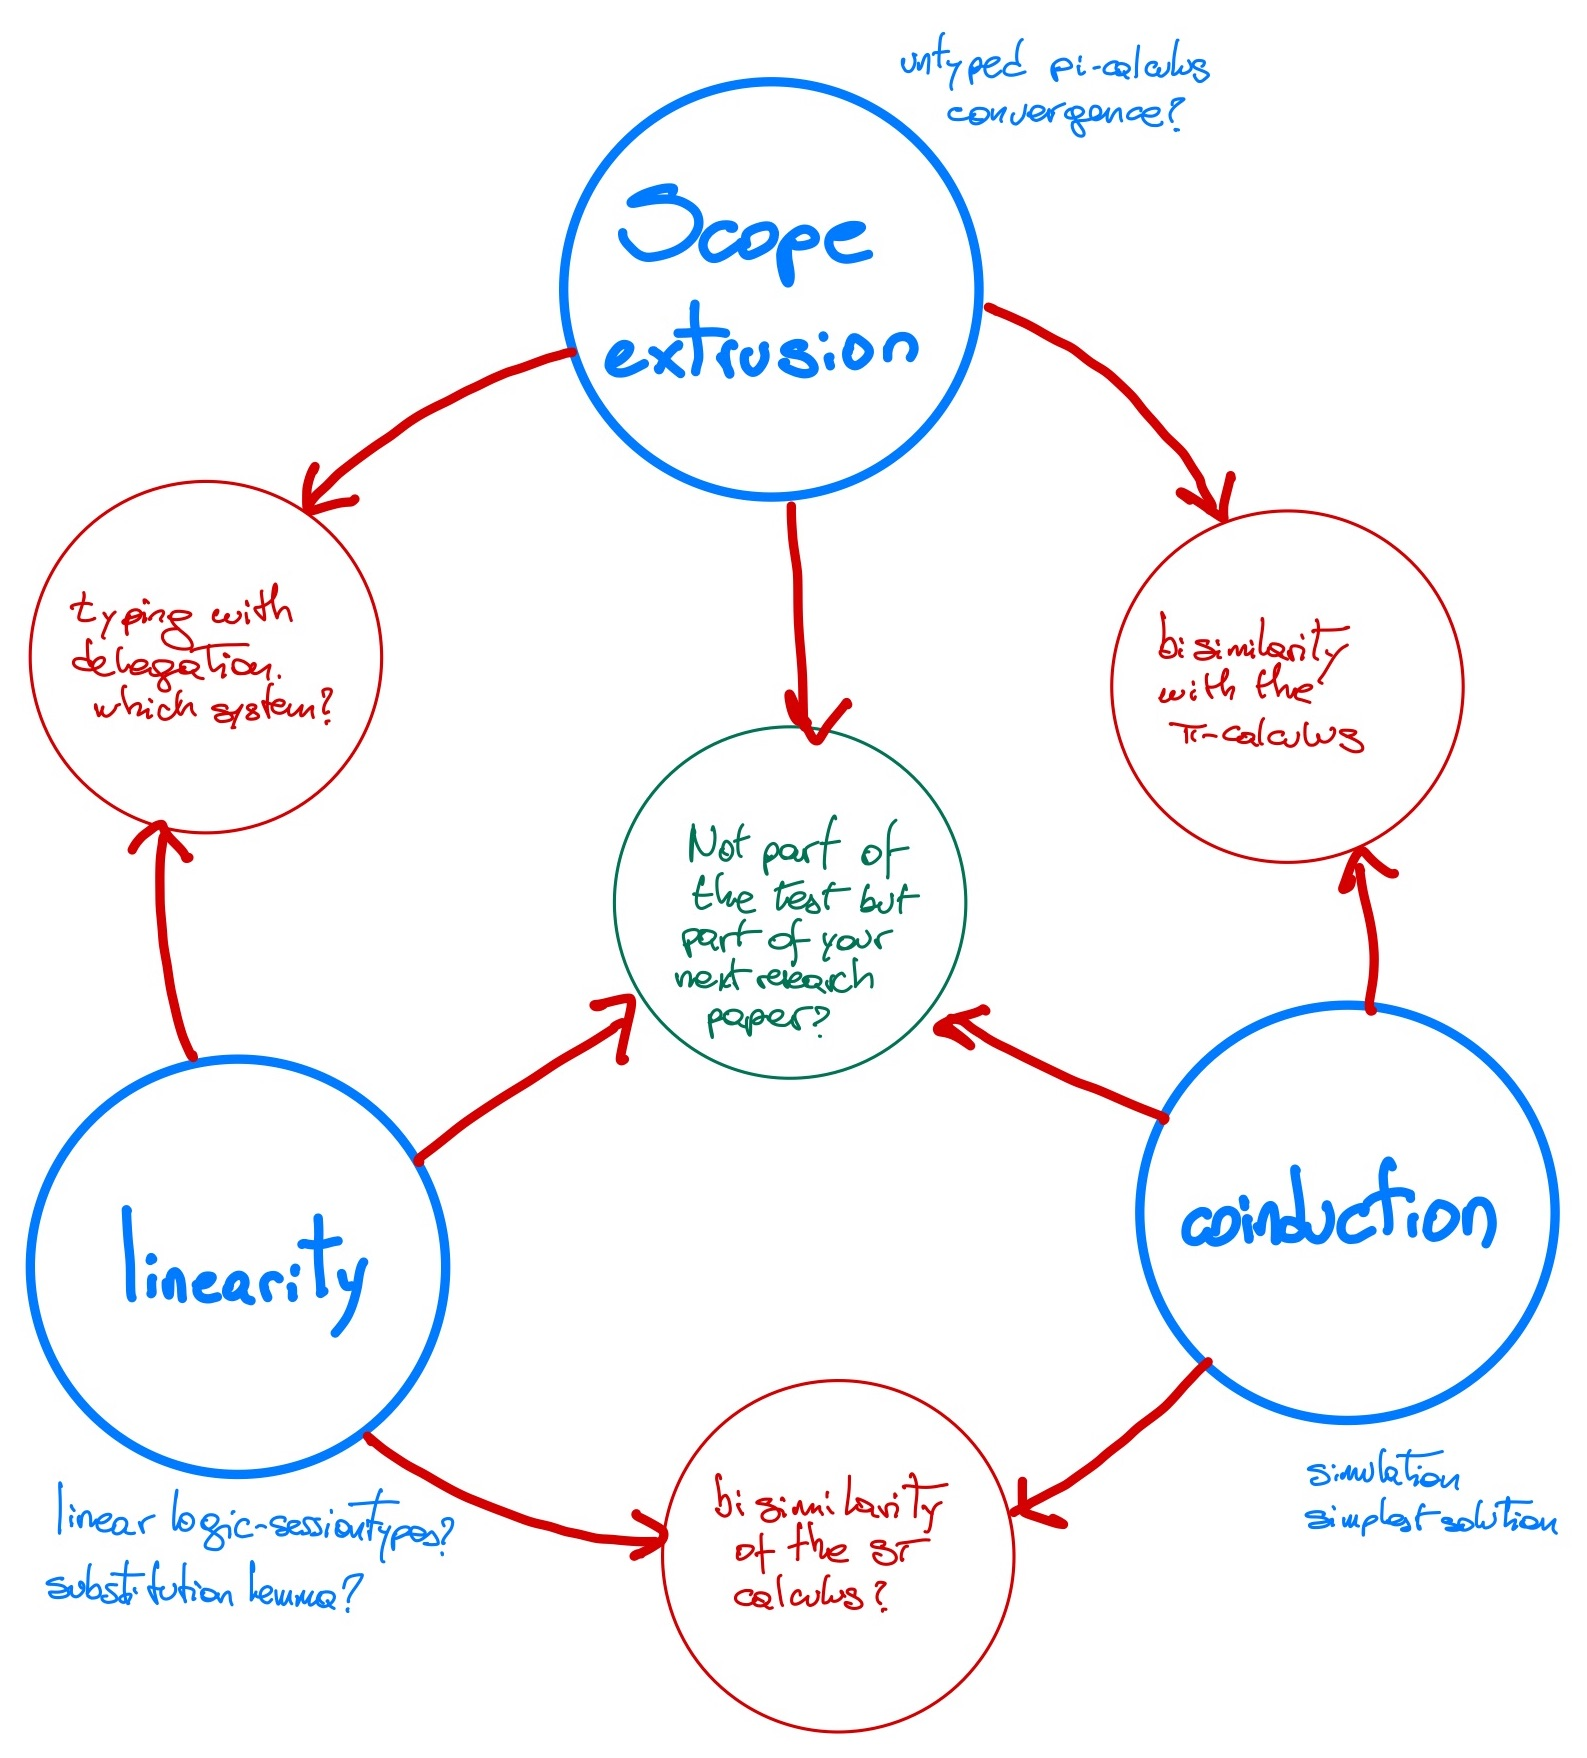
\includegraphics[width=0.75\textwidth]{images/benchmark.jpeg}
  \caption{The benchmark's big picture.}
  \label{fig:bigpic}
\end{figure}

The big picture for the benchmark can be seen in \cref{fig:bigpic}
where the three pillars (i.e.: concepts typically needed for process
calculus proofs) appear in blue, with some ideas of what to prove. And
a second step of combining the three aspects (for a total of six steps
for the whole benchmark), and of course the $+1$-step for the
combination of everything on the reader's next research papers.

\subsection{Name passing and scope extrusion}

\textbf{Problem idea}: A small proof about the untyped $\pi$-calculus.

\subsection{Linearity and behavioural type systems}

\textbf{Problem idea}: A small session type problem.

\subsection{Coinduction and reasoning about process algebras}

\textbf{Problem idea}: Something about traces, (bi)similarity, or
subtyping under non terminating problems in behavioural types.

\section{The solutions}\label{sec:solutions}

\subsection{A tutorial solution on paper}\label{sec:tutorial}

Probably the skeleton here and more details on an appendix.

\subsection{Flexibility in solving a challenge}

\section{Conclusion and related work} \label{sec:conclusion}

\bibliographystyle{plainnat}
\bibliography{references}

\label{lastpage01}

\end{document}
